% This is samplepaper.tex, a sample chapter demonstrating the
% LLNCS macro package for Springer Computer Science proceedings;
% Version 2.20 of 2017/10/04
%
\documentclass[runningheads]{llncs}
%
\usepackage{caption}  % For custom captions\usepackage{cite}     % For handling citations
\usepackage{amsmath}  % For mathematical features
\usepackage{graphicx}
\usepackage{booktabs}

\usepackage[colorlinks=true, urlcolor=blue, linkcolor=black]{hyperref}
% Used for displaying a sample figure. If possible, figure files should
% be included in EPS format.
%
% If you use the hyperref package, please uncomment the following line
% to display URLs in blue roman font according to Springer's eBook style:
% \renewcommand\UrlFont{\color{blue}\rmfamily}



\begin{document}
%
\title{Stroke Prediction Capstone Project}
%
%\titlerunning{Abbreviated paper title}
% If the paper title is too long for the running head, you can set
% an abbreviated paper title here
%
\author{Alvaro Quintero Gonzalez}
%
\authorrunning{A. Quintero Gonzalez.}
% First names are abbreviated in the running head.
% If there are more than two authors, 'et al.' is used.
%
\institute{Northwest Missouri State University, Maryville MO 64468, USA \\
\email{S573928@nwmissouri.edu and alvaroquintero28@yahoo.com}\\
}
%
\maketitle              % typeset the header of the contribution
%
\begin{abstract}
Stroke prediction is a critical area of research in healthcare, aiming to enhance preventative strategies and improve patient outcomes. This study investigates a comprehensive dataset collected from various healthcare sources, consisting of demographic, clinical, and lifestyle factors associated with stroke risk. The dataset encompasses attributes such as age, gender, blood pressure, cholesterol levels, body mass index (BMI), and lifestyle habits. "will finish at completion"

\keywords{Stroke Prediction \and Preventative Strategies \and Demographic Factors \and Predictive Modeling \and Machine Learning Algorithms}
\end{abstract}
%
%
%
\section{Introduction}

Strokes are a major health concern globally, recognized as one of the leading causes of disability and death. Occurring when blood flow to the brain is disrupted, it can lead to significant physical, cognitive, and emotional impairments in affected individuals. \cite{kaur2022retracted} The impact of strokes extends beyond the individual, affecting families and communities, and placing a substantial strain on healthcare systems. With the rising incidence of strokes associated with aging populations and the increasing prevalence of risk factors such as hypertension, obesity, and diabetes, there is an urgent need to focus on effective stroke prevention strategies. Prevention requires a multifaceted approach that includes public education, early identification of risk factors, and lifestyle modifications. Simple changes, such as adopting a balanced diet, engaging in regular physical activity, and managing underlying health conditions, can greatly reduce an individual's risk of stroke.\cite{doi:10.1161/STR.0000000000000375} Moreover, healthcare providers must play an active role in raising awareness about stroke prevention and ensuring that at-risk patients receive appropriate screenings and interventions. By promoting a comprehensive understanding of stroke risk factors, we can empower individuals to take charge of their health. This proactive approach not only aims to reduce the frequency of strokes but also facilitates overall public health awareness, fostering healthier communities. As advances in knowledge and strategies for stroke prevention, we can work towards a future where strokes are less frequent and their consequences are minimized \cite{sirisha2021awareness}.

\subsection{Define the Problem and Goals of This Capstone Project} 
This section discusses the goals of the proposed project. The primary focus of this capstone project is to develop a comprehensive understanding of stroke prediction and prevention strategies using data-driven approaches. Main goal consist of identifying key risk factors. By applying statistical analysis and machine learning techniques, it will determine which variables are most predictive of stroke occurrence. Further focus will evaluate performance of developed models in predicting stroke events, thereby providing valuable insights for early intervention. The project will propose targeted preventive strategies that can be implemented in community health programs therefore enhancing greater public awareness.

\subsubsection*{Project Links}
Key resources for this project provided below:

\begin{itemize}
    \item \href{https://github.com/alvaroquintero28/Capstone-Project-Report}{Capstone-Project-Report GitHub}
    \item \href{https://es.overleaf.com/read/zqgzcfntnwbz#9bc8ce}
    {Capstone Project Report Overleaf}
\end{itemize}

\subsection{The following are the phases of project implementation}

\begin{enumerate}
    \item Define the Problem and Objectives
    \begin{enumerate}
        \item Clearly articulate the specific questions and objectives of the analysis, focusing on how heart disease predictions can improve preventive measures for stroke patients.
         \item Identify key performance indicators (KPIs) to measure the success of the project. 
\end{enumerate}
\item  Literature Review and Background Research
\begin{enumerate}
    \item Conduct a thorough review of existing literature on heart disease, stroke rehabilitation, and predictive analytics in healthcare. 
    \item Gather insights into current best practices and identify gaps in the existing research that your project can address. 
\end{enumerate}
\item Data Collection
\begin{enumerate}
    \item Search for relevant datasets using the identified sources (e.g., ProjectPro, American Journal of Medicine) focusing on: 
    \begin{enumerate}
        \item Patient demographics 
        \item Medical history related to heart disease and strokes 
        \item Lifestyle factors (e.g., diet, exercise) 
        \item Laboratory test results (e.g., cholesterol levels, blood pressure) 
    \end{enumerate}
    \item Ensure that the data is reliable, accurate, and representative of the population you wish to study. 
\end{enumerate}
\item Data Pre-processing
    \begin{enumerate}
        \item Clean the data by handling missing values, outliers, and inconsistencies. 
        \item Perform data normalization or standardization if necessary. 
        \item Encode categorical variables to facilitate analysis in machine learning models. 
    \end {enumerate}
\item  Exploratory Data Analysis (EDA)
    \begin{enumerate}
        \item Analyze the dataset to uncover patterns and relationships between variables. 
        \item Use visualizations (graphs, plots) to represent findings and identify key risk factors associated with heart disease in stroke patients. 
    \end{enumerate}
\item Feature Selection
\begin{enumerate}
    \item Identify and select the most relevant features that influence heart disease predictions. 
    \item Use techniques like correlation analysis, recursive feature elimination (RFE), or machine learning algorithms to enhance feature selection. 
\end{enumerate}
\item Model Development
    \begin{enumerate}
        \item Choose appropriate machine learning models for prediction, such as: 
            \begin{enumerate}
                \item \item Logistic Regression
                \item Decision Trees 
                \item Random Forest 
                \item Support Vector Machines 
                \item Neural Networks 
            \end{enumerate}
        \item Split the dataset into training and testing sets for model evaluation. 
    \end{enumerate}
\item Model Training and Tuning
    \begin{enumerate}
        \item Train the selected models on the training dataset. 
        \item Optimize model performance using techniques like hyperparameter tuning and cross-validation to prevent overfitting. 
    \end{enumerate}
\item Model Evaluation
\begin{enumerate}
    \item Assess the accuracy and effectiveness of the models using the testing dataset. 
    \item Use evaluation metrics such as accuracy, precision, recall, F1 score, and the ROC-AUC curve to measure performance. 
    \item Compare the performance of different models to select the best one. 
\end{enumerate}
\item Conclusion
\begin{enumerate}
    \item Interpret Results
        \begin{enumerate}
            \item Analyze the results of the best-performing model to understand the impact of various factors on heart disease predictions. 
            \item Provide actionable insights and recommendations for preventing heart disease in stroke patients based on the findings. 
        \end{enumerate}
\item Discussion of the limitations
\item Ideas for future work.
\end{enumerate}

\section{Literature Review and Background Research}
Numerous studies have identified effective preventive measures for reducing the risk of stroke, emphasizing both management of hypertension and lifestyle interventions. \cite{sirisha2021awareness} Hypertension is the most significant modifiable risk factor for stroke, and studies have shown that controlling blood pressure through lifestyle changes, such as a healthy diet, regular physical activity, reducing sodium intake, smoking cessation, and adhering to prescribed antihypertensive medications can significantly lower the likelihood of experiencing a stroke. Maintaining blood pressure within a normal range (typically less than 120/80 mmHg) is crucial in preventing both ischemic and hemorrhagic strokes, making it the most critical focus in stroke prevention efforts. \cite{doi:10.1161/STR.0000000000000375} Combined, these research findings underscore the importance of a multifaceted approach to stroke prevention that integrates medical treatment with proactive lifestyle changes.

\subsection{Limitations}
The healthcare stroke prevention dataset and the well-being and lifestyle dataset each have inherent limitations that may affect the comprehensiveness and applicability of their findings. Firstly, the stroke prevention dataset may suffer from issues related to sample size and demographic representation, potentially limiting the generalizability of the results across diverse populations. Additionally, the accuracy of self-reported data regarding lifestyle factors in the well-being and lifestyle dataset may be compromised by social desirability bias, where participants might under-report unhealthy behaviors or exaggerate healthy ones. Furthermore, the transient nature of lifestyle habits makes it challenging to capture accurate and stable data over time, potentially leading to discrepancies in understanding long-term behavior trends.

\section{Data}
Data collection for this analysis involved two comprehensive datasets sourced from Kaggle: the Wellbeing and Lifestyle Data and the Healthcare Dataset on Stroke Data. The Wellbeing and Lifestyle Data dataset encompasses a variety of factors influencing individual health and well-being, such as lifestyle choices. It features demographic information, including age, gender, and socioeconomic status, facilitating an understanding of how these variables correlate with reported well-being outcomes. The Healthcare Dataset and Stroke Data, on the other hand, presents critical health metrics and conditions related to stroke incidents among patients. By merging insights from these two datasets, a more comprehensive picture of lifestyle influences on health outcomes can be constructed, enabling a deeper exploration of the relationships between well-being, lifestyle choices, and stroke risk.


\subsection{Dataset Variable Attributes}

The following tables summarize the variables in the datasets, including their descriptions, data types, and possible values. These attributes are essential for understanding the data collected and for any subsequent analysis.

\begin{table}  
\centering    
\caption{Selected Variable Descriptions}\label{tab1} 

\begin{tabular}{|l|l|l|} 
\hline     

\textbf{Variable Name} & \textbf{Description} & \textbf{Possible Values} \\        \hline        age & Age of the patient in years & Whole numbers (e.g., 0, 1, 25, 60) \\        \hline        gender & Gender of the patient & "Male", "Female", "Other" \\        \hline        hypertension & Indicates if the patient has hypertension & 0 (No), 1 (Yes) \\        \hline        heart\_disease & Indicates if the patient has heart disease & 0 (No), 1 (Yes) \\        \hline        ever\_married & Indicates if the patient has ever been married & "No", "Yes" \\        \hline        work\_type & Type of employment of the patient & "children", "Govt job", "Never worked", 
"Private", "Self-employed" \\        \hline        bmi & Body Mass Index of the patient & Positive floats (e.g., 18.5, 30.0) \\        \hline        smoking\_status & Indicates the smoking status of the patient & "formerly smoked", "smokes"\\        
\hline    
\end{tabular}    
\end{table}

\begin{table}[ht]
    \centering
    \caption{Daily Stress Levels}\label{tab1}
    \begin{tabular}{|l|l|l|}
        \hline
        \textbf{Stress Level (0-10)} & \textbf{Count} \\ 
        \hline
        0.00 - 0.25 & 676 \\ 
        1.00 - 1.25 & 2,478 \\ 
        2.00 - 2.25 & 3,407 \\ 
        3.00 - 3.25 & 4,398 \\ 
        4.00 - 4.25 & 2,960 \\ 
        4.75 - 5.00 & 2,052 \\ 
        \hline
    \end{tabular}
\end{table}

\begin{table}[ht]
    \centering
    \caption{Typical Sleep Hours}\label{tab1}
    \begin{tabular}{|l|l|l|}
        \hline
        \textbf{Sleep Hours (0-10)} & \textbf{Count} \\ 
        \hline
        1.00 - 1.45 & 18 \\ 
        1.90 - 2.35 & 21 \\ 
        2.80 - 3.25 & 49 \\ 
        3.70 - 4.15 & 252 \\ 
        4.60 - 5.05 & 1,025 \\ 
        5.95 - 6.40 & 3,397 \\ 
        6.85 - 7.30 & 5,566 \\ 
        7.75 - 8.20 & 4,324 \\ 
        8.65 - 9.10 & 987 \\ 
        9.55 - 10.00 & 333 \\ 
        \hline
    \end{tabular}
\end{table}

\begin{table}
    \centering
    \caption{Income Sufficiency}\label{tab1}
    \begin{tabular}{|l|l|l|}
        \hline
        \textbf{Income Sufficiency} & \textbf{Count} \\ 
        \hline
        1.00 - 1.05 & 4,329 \\ 
        1.95 - 2.00 & 11,643 \\ 
        \hline
    \end{tabular}

\end{table}


\begin{table}[ht]
    \centering
    \caption{Demographic Breakdown by Age}\label{tab1}
    \begin{tabular}{|l|l|l|}
        \hline
        \textbf{Age Group} & \textbf{Percentage} \\ 
        \hline
        21 to 35 & 38\% \\ 
        36 to 50 & 29\% \\ 
        Other & 33\% \\ 
        \hline
    \end{tabular}
\end{table}
\clearpage

\begin{table}[h]
    \centering
    \caption{Gender Breakdown}\label{tab1}
    \begin{tabular}{|l|l|l|}
        \hline
        \textbf{Gender} & \textbf{Percentage} \\ 
        \hline
        Female & 62\% \\ 
        Male & 38\% \\ 
        \hline
    \end{tabular}
\end{table}

\begin{figure}
    \centering
    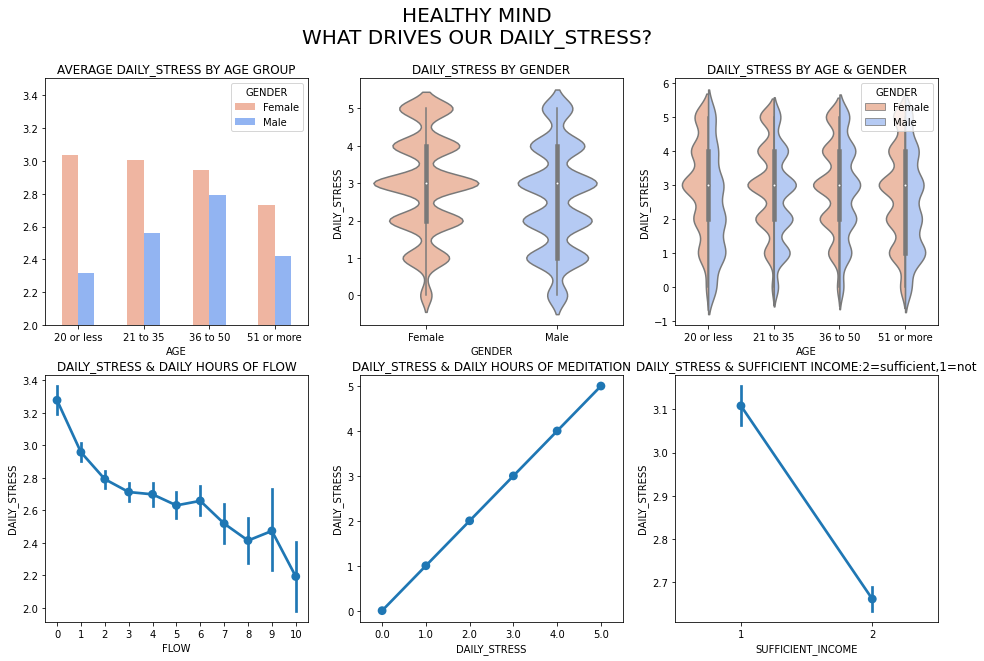
\includegraphics[width=1.2\linewidth]{__results___16_0.png}
    \caption{Summary of Daily Stress}\cite{Work-Life}
    \label{fig:enter-label}
\end{figure}

\section{Cleaning}
Data cleaning is a crucial step in preparing data for analysis, ensuring that the datasets are accurate, consistent, and complete such as in Table 1, which summarizes the descriptions and possible values for key attributes. Inconsistencies were identified and rectified in the data, particularly for categorical variables like gender and the presence of health conditions such as hypertension and heart disease, which are coded as binary values (0 for "No" and 1 for "Yes"). Additionally, the numerical data, including the Body Mass Index (BMI) and income sufficiency scores, were examined to ensure they fell within realistic ranges. For continuous variables like daily stress levels and sleep hours, frequency distributions were tabulated, as demonstrated in subsequent tables, to check for outliers. This included examining stress levels, which were recorded in intervals, revealing patterns in the counts associated with each level (Table 2). Demographic distributions were focused on, such as age and gender breakdowns (Tables 4 and 5), confirming their representation matched expectations based on the source population. By employing these data cleaning techniques, it improved the reliability of analysis and enhanced the validity of the findings regarding daily stress influences. For instance, the graphical summary shown in Figure \ref{fig:Healthy Mind What Drives Our Daily Stress} visually represents the analyzed data, indicating significant relationships that deserve further exploration.

\subsection{Individualized Dataset A.}

Data cleaning was a critical step in analyzing the Work-Life Balance Survey, which encompasses over 10,000 responses to a global work-life questionnaire. Initially, the dataset is imported using Pandas, and preliminary checks reveal various data types across its 23 columns, including responses pertaining to lifestyle habits and work-life balance indicators. As part of the cleaning process, certain categorical values are standardized; for example, the age category "Less than 20" is replaced with "20 or less" for consistency. Additionally, columns such as 'DAILY STRESS' are converted to numeric types to facilitate statistical analysis, with errors handled through coercion to manage any non-numeric values effectively. Duplicate entries are examined to ensure data integrity, while any missing values are identified, particularly in key variables that influence analysis outcomes. Descriptive summaries are generated to provide insights into the data distribution and identify any anomalies. This cleaning process prepares the dataset for robust exploratory analysis, allowing clearer insights into the factors that shape work-life balance and their implications for improving overall well-being.

\subsection{Individualized Dataset B.}

Data cleaning was a crucial step in preparing the stroke prediction dataset for analysis and model building. Initially, the dataset is loaded using Pandas, revealing 5,110 entries and 11 columns, with notable missing values in the 'bmi' column (201 nulls). Data types are assessed, and it is observed that the dataset contains both categorical and numerical features. Handling missing values is prioritized, specifically through K-Nearest Neighbors (KNN) imputation for the 'bmi' field after encoding categorical variables using Label Encoding. The 'stroke' column is converted into binary values for better interpretability. Correlation analysis is conducted, highlighting key features like age, hypertension, and heart disease that demonstrate significant relationships with stroke occurrence. Furthermore, data splitting is performed to separate the features and target variable, followed by Min-Max scaling to ensure all numerical inputs are normalized within a specified range. Recognizing class imbalance, Techniques such as SMOTE (Synthetic Minority Over-sampling Technique) are employed to balance the dataset before fitting several machine learning models, enhancing predictive capabilities and improving overall model performance. This structured cleaning pipeline ultimately sets the stage for effective exploratory analysis and accurate predictive modeling.

\section{Exploratory Data Analysis}


\clearpage
\nocite{*}
\bibliographystyle{splncs04}
\bibliography{mybibliography}


%


\end{document}
